\documentclass[11pt,a4paper]{report}

% ============================================
% PACKAGES
% ============================================
\usepackage[utf8]{inputenc}
\usepackage[T1]{fontenc}
\usepackage{lmodern}
\usepackage[margin=2.5cm]{geometry}
\usepackage{graphicx}
\usepackage{xcolor}
\usepackage{tikz}
\usetikzlibrary{shapes.geometric, arrows.meta, positioning, calc, decorations.pathreplacing, patterns, shadows}
\usepackage{amsmath,amssymb}
\usepackage{booktabs}
\usepackage{array}
\usepackage{longtable}
\usepackage{fancyhdr}
\usepackage{hyperref}
\usepackage{algorithm}
\usepackage{algpseudocode}
\usepackage{listings}
\usepackage{tcolorbox}
\tcbuselibrary{skins,breakable}
\usepackage{enumitem}
\usepackage{multicol}

% ============================================
% LISTINGS CONFIGURATION
% ============================================
\lstset{
    basicstyle=\small\ttfamily,
    keywordstyle=\color{primaryblue}\bfseries,
    commentstyle=\color{secondarygreen}\itshape,
    stringstyle=\color{accentorange},
    numberstyle=\tiny\color{gray},
    backgroundcolor=\color{codebg},
    frame=single,
    framerule=0.5pt,
    rulecolor=\color{primaryblue!50},
    breaklines=true,
    breakatwhitespace=true,
    tabsize=4,
    showstringspaces=false,
    captionpos=t,
    aboveskip=10pt,
    belowskip=10pt,
    xleftmargin=5pt,
    xrightmargin=5pt,
    framexleftmargin=5pt,
    framexrightmargin=5pt
}

% ============================================
% COLORS
% ============================================
\definecolor{primaryblue}{RGB}{0,82,147}
\definecolor{secondarygreen}{RGB}{0,128,0}
\definecolor{accentorange}{RGB}{230,126,34}
\definecolor{quantumpurple}{RGB}{128,0,128}
\definecolor{hardwarered}{RGB}{192,57,43}
\definecolor{lightgray}{RGB}{245,245,245}
\definecolor{codebg}{RGB}{248,248,248}

% ============================================
% HEADER/FOOTER
% ============================================
\pagestyle{fancy}
\fancyhf{}
\fancyhead[L]{\leftmark}
\fancyhead[R]{\thepage}
\fancyfoot[C]{\small Post-Quantum Cryptography \& Hardware Acceleration}
\renewcommand{\headrulewidth}{0.4pt}
\renewcommand{\footrulewidth}{0.4pt}

% ============================================
% CUSTOM BOXES
% ============================================
\newtcolorbox{keypoint}[1][]{
    colback=primaryblue!5,
    colframe=primaryblue,
    fonttitle=\bfseries,
    title=#1,
    rounded corners,
    boxrule=1pt
}

\newtcolorbox{warningbox}[1][]{
    colback=accentorange!10,
    colframe=accentorange,
    fonttitle=\bfseries,
    title=#1,
    rounded corners,
    boxrule=1pt
}

\newtcolorbox{infobox}[1][]{
    colback=secondarygreen!5,
    colframe=secondarygreen,
    fonttitle=\bfseries,
    title=#1,
    rounded corners,
    boxrule=1pt
}

% ============================================
% HYPERREF SETUP
% ============================================
\hypersetup{
    colorlinks=true,
    linkcolor=primaryblue,
    urlcolor=primaryblue,
    citecolor=secondarygreen
}

% ============================================
% DOCUMENT INFO
% ============================================
\title{
    \vspace{-1cm}
    \begin{tikzpicture}[remember picture, overlay]
        \fill[primaryblue] (current page.north west) rectangle ([yshift=-6cm]current page.north east);
    \end{tikzpicture}
    \vspace{2cm}
    {\color{white}\Huge\bfseries Post-Quantum Cryptography}\\[0.5cm]
    {\color{white}\Huge\bfseries \&}\\[0.5cm]
    {\color{white}\Huge\bfseries Hardware Acceleration}\\[1cm]
    {\color{white}\Large GPU and FPGA-Based Compression}\\[0.5cm]
    {\color{white}\large A Comprehensive Guide}
}
\author{
    \vspace{2cm}\\
    \textbf{Abdessamad JAOUAD}\\
    M2 Big Data \& IoT\\
    ENSAM Casablanca
}
\date{\today}

\begin{document}

% ============================================
% TITLE PAGE
% ============================================
\begin{titlepage}
\centering
\vspace*{1cm}

% Header decoration
\begin{tikzpicture}[remember picture, overlay]
    \fill[primaryblue] (current page.north west) rectangle ([yshift=-7cm]current page.north east);
    % Quantum circuit decoration
    \foreach \i in {1,...,5} {
        \draw[white, thick, opacity=0.3] ([xshift=\i*3cm, yshift=-2cm]current page.north west) -- ++(0,-3cm);
        \node[circle, fill=white, opacity=0.3, minimum size=8pt] at ([xshift=\i*3cm, yshift=-3.5cm]current page.north west) {};
    }
\end{tikzpicture}

\vspace{5cm}
{\color{black}\Huge\bfseries Post-Quantum Cryptography}\\[0.3cm]
{\color{black}\Huge\bfseries \&}\\[0.3cm]
{\color{black}\Huge\bfseries Hardware Acceleration}\\[0.8cm]
{\color{black}\Large GPU and FPGA-Based Compression}\\[0.3cm]
{\color{black}\normalsize A Comprehensive Guide for Future-Proof Computing}
\vspace{3cm}

% Central illustration
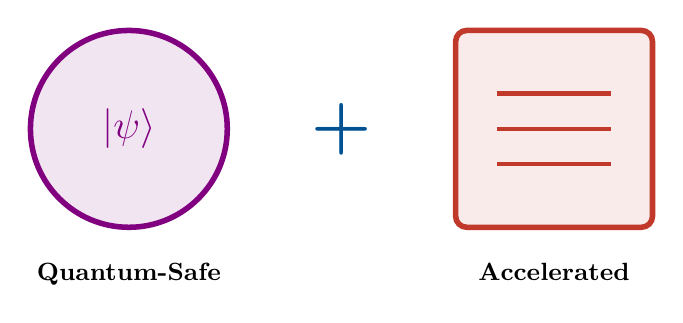
\begin{tikzpicture}[scale=0.9]
    % Quantum symbol
    \node[circle, draw=quantumpurple, line width=2pt, minimum size=2.5cm, fill=quantumpurple!10] (quantum) at (-3,0) {};
    \node at (-3,0) {\color{quantumpurple}\Large $|\psi\rangle$};
    \node[below=0.3cm of quantum] {\small\textbf{Quantum-Safe}};
    
    % Plus sign
    \node at (0,0) {\Huge\color{primaryblue}\textbf{+}};
    
    % Hardware symbol
    \node[rectangle, draw=hardwarered, line width=2pt, minimum size=2.5cm, fill=hardwarered!10, rounded corners] (hw) at (3,0) {};
    \draw[hardwarered, line width=1.5pt] (2.2,0.5) -- (3.8,0.5);
    \draw[hardwarered, line width=1.5pt] (2.2,0) -- (3.8,0);
    \draw[hardwarered, line width=1.5pt] (2.2,-0.5) -- (3.8,-0.5);
    \node[below=0.3cm of hw] {\small\textbf{Accelerated}};
\end{tikzpicture}

\vspace{2cm}

\rule{0.6\textwidth}{0.5pt}\\[0.5cm]
{\Large\textbf{Abdessamad JAOUAD}}\\[0.3cm]
{\large M2 Big Data \& IoT}\\[0.2cm]
{\large ENSAM Casablanca}\\[1cm]
{\large \today}

\end{titlepage}

% ============================================
% TABLE OF CONTENTS
% ============================================
\tableofcontents
\newpage

% ============================================
% CHAPTER 1: INTRODUCTION
% ============================================
\chapter{Introduction}

\section{The Quantum Threat}

The advent of \textbf{quantum computing} poses an existential threat to modern cryptography. Algorithms like \textbf{Shor's algorithm} can break RSA, ECC, and other public-key systems in polynomial time.

\begin{keypoint}[Harvest Now Decrypt Later Attack]
Adversaries are already collecting encrypted data today, planning to decrypt it once quantum computers become available. This makes post-quantum migration \textbf{urgent}.
\end{keypoint}

\subsection{Timeline Estimates}

\begin{center}
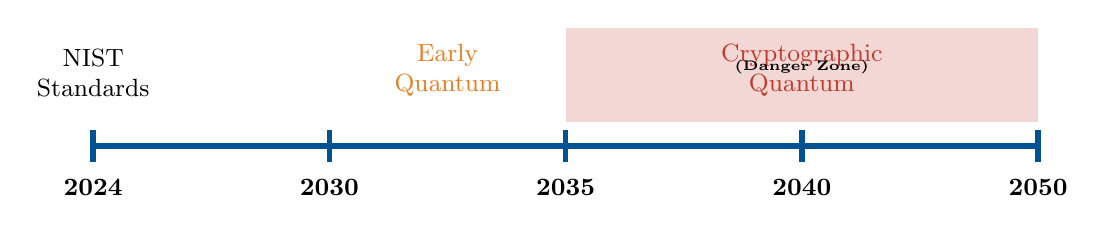
\begin{tikzpicture}[scale=1, transform shape]
    % Timeline
    \draw[line width=2pt, primaryblue] (0,0) -- (12,0);
    
    % Years
    \foreach \x/\year in {0/2024, 3/2030, 6/2035, 9/2040, 12/2050} {
        \draw[primaryblue, line width=2pt] (\x,-0.2) -- (\x,0.2);
        \node[below] at (\x,-0.3) {\small\textbf{\year}};
    }
    
    % Events
    \node[above, align=center, font=\small] at (0,0.5) {NIST\\Standards};
    \node[above, align=center, font=\small, text=accentorange] at (4.5,0.5) {Early\\Quantum};
    \node[above, align=center, font=\small, text=hardwarered] at (9,0.5) {Cryptographic\\Quantum};
    
    % Danger zone
    \fill[hardwarered, opacity=0.2] (6,0.3) rectangle (12,1.5);
    \node[font=\tiny] at (9,1) {\textbf{(Danger Zone)}};
\end{tikzpicture}
\end{center}

\section{The Performance Challenge}

Post-quantum algorithms have significantly \textbf{larger key sizes} and \textbf{slower operations} than classical cryptography. Hardware acceleration becomes essential.

\begin{table}[h]
\centering
\caption{Key Size Comparison: Classical vs. Post-Quantum}
\begin{tabular}{@{}lccc@{}}
\toprule
\textbf{Algorithm} & \textbf{Type} & \textbf{Public Key} & \textbf{Private Key} \\
\midrule
RSA-2048 & Classical & 256 B & 1.2 KB \\
ECDSA P-256 & Classical & 64 B & 32 B \\
\midrule
ML-KEM-768 & PQC (Lattice) & 1,184 B & 2,400 B \\
ML-DSA-65 & PQC (Lattice) & 1,952 B & 4,032 B \\
SLH-DSA-128s & PQC (Hash) & 32 B & 64 B \\
\bottomrule
\end{tabular}
\end{table}

\section{Hardware Acceleration Solutions}

Two main approaches exist for accelerating cryptographic and compression workloads:

\begin{center}
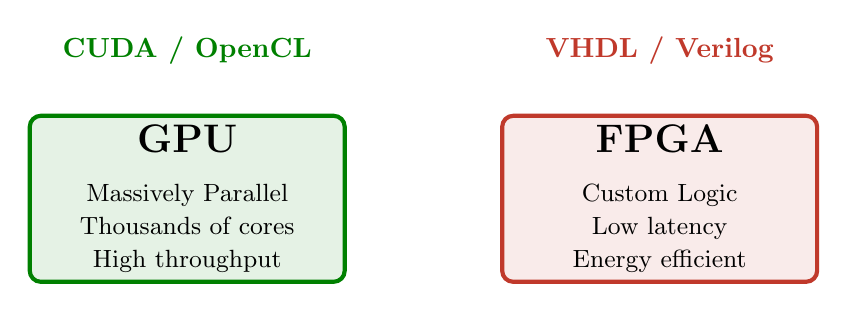
\begin{tikzpicture}[
    box/.style={rectangle, draw=#1, line width=1.5pt, fill=#1!10, 
                minimum width=4cm, minimum height=2cm, rounded corners, align=center}
]
    % GPU Box
    \node[box=secondarygreen] (gpu) at (-3,0) {
        \textbf{\Large GPU}\\[0.2cm]
        \small Massively Parallel\\
        \small Thousands of cores\\
        \small High throughput
    };
    
    % FPGA Box
    \node[box=hardwarered] (fpga) at (3,0) {
        \textbf{\Large FPGA}\\[0.2cm]
        \small Custom Logic\\
        \small Low latency\\
        \small Energy efficient
    };
    
    % Labels
    \node[above=0.5cm of gpu, font=\bfseries\color{secondarygreen}] {CUDA / OpenCL};
    \node[above=0.5cm of fpga, font=\bfseries\color{hardwarered}] {VHDL / Verilog};
\end{tikzpicture}
\end{center}

\section{Document Overview}

This guide covers two critical future trends in computing:

\begin{enumerate}[leftmargin=*]
    \item \textbf{Post-Quantum Cryptography (PQC)} -- Cryptographic algorithms resistant to quantum attacks
    \item \textbf{Hardware Acceleration} -- GPU and FPGA-based acceleration for compression and cryptography
\end{enumerate}

\begin{infobox}[Chapter Roadmap]
\begin{itemize}[leftmargin=*, nosep]
    \item \textbf{Chapter 2:} Post-Quantum Cryptography Fundamentals
    \item \textbf{Chapter 3:} PQC Algorithm Families
    \item \textbf{Chapter 4:} NIST PQC Standards
    \item \textbf{Chapter 5:} GPU Architecture \& CUDA
    \item \textbf{Chapter 6:} OpenCL \& Cross-Platform Computing
    \item \textbf{Chapter 7:} FPGA Architecture \& Programming
    \item \textbf{Chapter 8:} Hardware-Accelerated Compression
    \item \textbf{Chapter 9:} Conclusion \& Future Directions
\end{itemize}
\end{infobox}

\section{Why This Matters}

\begin{warningbox}[Critical Takeaway]
The intersection of \textbf{post-quantum security} and \textbf{hardware acceleration} is not optional---it's essential for any system that needs to remain secure and performant in the coming decades.
\end{warningbox}

% ============================================
% CHAPTER 2: PQC FUNDAMENTALS
% ============================================
\chapter{Post-Quantum Cryptography Fundamentals}

\section{What is Post-Quantum Cryptography?}

\textbf{Post-Quantum Cryptography (PQC)} refers to cryptographic algorithms designed to resist attacks from both classical and quantum computers.

\begin{keypoint}[Key Distinction]
PQC algorithms run on \textbf{classical computers}---they don't require quantum hardware. They're simply designed to resist quantum attacks.
\end{keypoint}

\section{Why Current Cryptography Fails}

\subsection{Shor's Algorithm}

Shor's algorithm (1994) can efficiently solve two hard problems:

\begin{center}
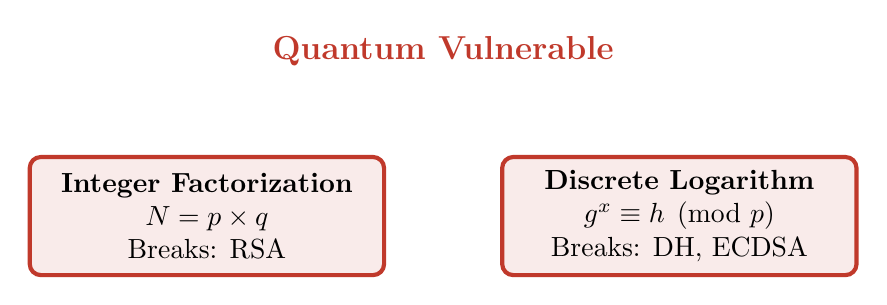
\begin{tikzpicture}[
    problem/.style={rectangle, draw=hardwarered, line width=1.5pt, fill=hardwarered!10, 
                    minimum width=4.5cm, minimum height=1.5cm, rounded corners, align=center}
]
    \node[problem] (factor) at (-3,0) {\textbf{Integer Factorization}\\$N = p \times q$\\Breaks: RSA};
    \node[problem] (dlog) at (3,0) {\textbf{Discrete Logarithm}\\$g^x \equiv h \pmod{p}$\\Breaks: DH, ECDSA};
    
    \node[above=1cm of factor, xshift=3cm, font=\large\bfseries\color{hardwarered}] {Quantum Vulnerable};
\end{tikzpicture}
\end{center}

\subsection{Complexity Comparison}

\begin{table}[h]
\centering
\caption{Time Complexity: Classical vs Quantum}
\begin{tabular}{@{}lcc@{}}
\toprule
\textbf{Problem} & \textbf{Classical} & \textbf{Quantum (Shor)} \\
\midrule
Factoring $n$-bit integer & $O(e^{n^{1/3}})$ & $O(n^3)$ \\
Discrete Log & $O(e^{n^{1/3}})$ & $O(n^3)$ \\
\bottomrule
\end{tabular}
\end{table}

\begin{warningbox}[Exponential to Polynomial]
Shor's algorithm reduces \textbf{exponential} problems to \textbf{polynomial} time---a catastrophic break for RSA and ECC.
\end{warningbox}

\section{Grover's Algorithm}

Grover's algorithm provides a \textbf{quadratic speedup} for searching unsorted databases:

\begin{itemize}[leftmargin=*, nosep]
    \item Classical search: $O(N)$
    \item Quantum search: $O(\sqrt{N})$
\end{itemize}

\textbf{Impact on symmetric crypto:} AES-128 becomes effectively AES-64. Solution: \textbf{double key sizes} (AES-256).

\section{Mathematical Foundations of PQC}

PQC relies on problems believed to be hard for \textit{both} classical and quantum computers:

\begin{center}
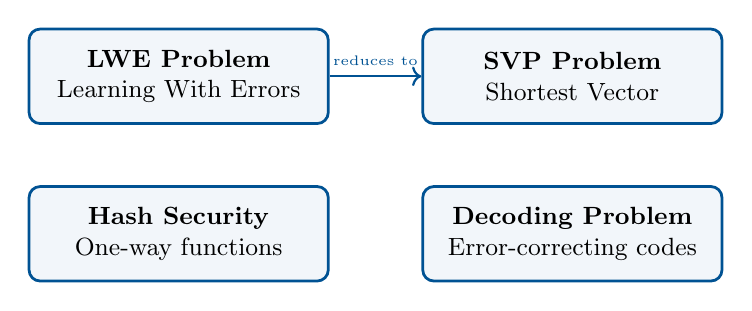
\begin{tikzpicture}[
    node distance=0.8cm,
    box/.style={rectangle, draw=primaryblue, line width=1pt, fill=primaryblue!5, 
                minimum width=3.8cm, minimum height=1.2cm, rounded corners, align=center, font=\small}
]
    \node[box] (lwe) at (0,2) {\textbf{LWE Problem}\\Learning With Errors};
    \node[box] (svp) at (5,2) {\textbf{SVP Problem}\\Shortest Vector};
    \node[box] (hash) at (0,0) {\textbf{Hash Security}\\One-way functions};
    \node[box] (code) at (5,0) {\textbf{Decoding Problem}\\Error-correcting codes};
    
    \draw[->, thick, primaryblue] (lwe) -- node[above, font=\tiny] {reduces to} (svp);
\end{tikzpicture}
\end{center}

\section{Security Levels}

NIST defines 5 security levels based on equivalent classical security:

\begin{table}[h]
\centering
\caption{NIST Security Levels}
\begin{tabular}{@{}clc@{}}
\toprule
\textbf{Level} & \textbf{Equivalent Security} & \textbf{Bits} \\
\midrule
1 & AES-128 key search & 128 \\
2 & SHA-256 collision & 128 \\
3 & AES-192 key search & 192 \\
4 & SHA-384 collision & 192 \\
5 & AES-256 key search & 256 \\
\bottomrule
\end{tabular}
\end{table}

% ============================================
% CHAPTER 3: PQC ALGORITHM FAMILIES
% ============================================
\chapter{PQC Algorithm Families}

Post-quantum algorithms are grouped into families based on their underlying mathematical problems.

\section{Overview of Algorithm Families}

\begin{center}
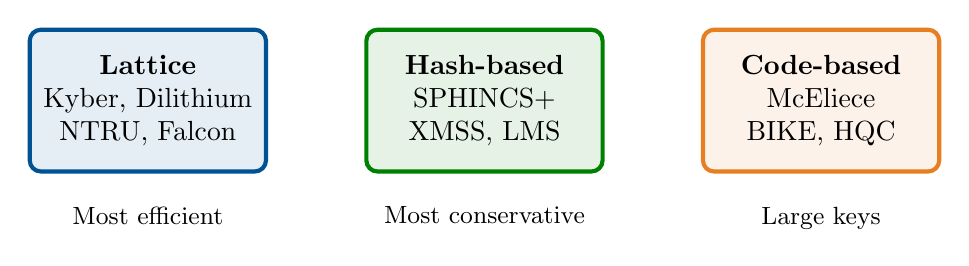
\begin{tikzpicture}[
    family/.style={rectangle, draw=#1, line width=1.5pt, fill=#1!10, 
                   minimum width=3cm, minimum height=1.8cm, rounded corners, align=center},
    scale=0.95
]
    % Row 1
    \node[family=primaryblue] (lattice) at (0,0) {\textbf{Lattice}\\Kyber, Dilithium\\NTRU, Falcon};
    \node[family=secondarygreen] (hash) at (4.5,0) {\textbf{Hash-based}\\SPHINCS+\\XMSS, LMS};
    \node[family=accentorange] (code) at (9,0) {\textbf{Code-based}\\McEliece\\BIKE, HQC};
    
    % Labels
    \node[below=0.3cm of lattice, font=\small] {Most efficient};
    \node[below=0.3cm of hash, font=\small] {Most conservative};
    \node[below=0.3cm of code, font=\small] {Large keys};
\end{tikzpicture}
\end{center}

\section{Lattice-Based Cryptography}

\subsection{What is a Lattice?}

A \textbf{lattice} is a regular grid of points in $n$-dimensional space, generated by a set of basis vectors.

\begin{center}
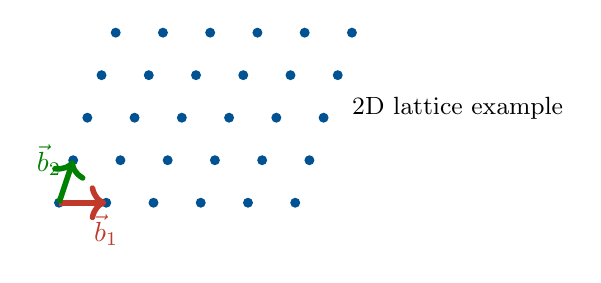
\begin{tikzpicture}[scale=0.6]
    % Draw lattice points
    \foreach \x in {0,1,2,3,4,5} {
        \foreach \y in {0,1,2,3,4} {
            \fill[primaryblue] (\x+0.3*\y, \y*0.9) circle (3pt);
        }
    }
    % Basis vectors
    \draw[->, line width=2pt, hardwarered] (0,0) -- (1,0) node[below] {$\vec{b}_1$};
    \draw[->, line width=2pt, secondarygreen] (0,0) -- (0.3,0.9) node[left] {$\vec{b}_2$};
    
    \node[right] at (6,2) {\small 2D lattice example};
\end{tikzpicture}
\end{center}

\subsection{Hard Lattice Problems}

\begin{enumerate}[leftmargin=*, nosep]
    \item \textbf{SVP} (Shortest Vector Problem): Find the shortest non-zero vector
    \item \textbf{CVP} (Closest Vector Problem): Find the closest lattice point to a target
    \item \textbf{LWE} (Learning With Errors): Distinguish noisy linear equations from random
\end{enumerate}

\subsection{LWE Problem Explained}

Given samples of the form:
\[
(\mathbf{a}_i, b_i = \langle \mathbf{a}_i, \mathbf{s} \rangle + e_i) \mod q
\]

Where $\mathbf{s}$ is secret and $e_i$ is small noise. \textbf{Goal:} Recover $\mathbf{s}$.

\begin{infobox}[Why LWE is Hard]
The noise $e_i$ prevents simple linear algebra solutions. Without noise, solving is trivial. With noise, it becomes as hard as worst-case lattice problems.
\end{infobox}

\section{Hash-Based Signatures}

Hash-based signatures rely \textit{only} on the security of hash functions---the most conservative assumption.

\subsection{One-Time Signatures (OTS)}

\begin{center}
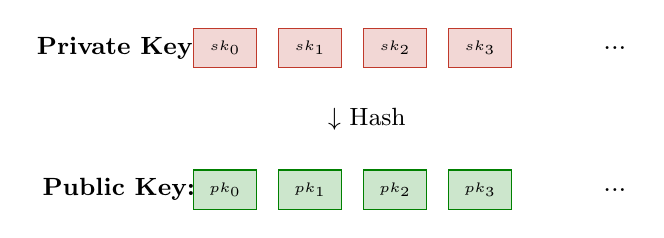
\begin{tikzpicture}[scale=0.9]
    % Private key (seeds)
    \node[font=\small\bfseries] at (-1.5, 2) {Private Key:};
    \foreach \i in {0,...,3} {
        \node[rectangle, draw=hardwarered, fill=hardwarered!20, minimum width=0.8cm, minimum height=0.5cm] 
            (sk\i) at (\i*1.2, 2) {\tiny $sk_\i$};
    }
    \node at (5.5, 2) {...};
    
    % Hash function
    \node[font=\small] at (2, 1) {$\downarrow$ Hash};
    
    % Public key
    \node[font=\small\bfseries] at (-1.5, 0) {Public Key:};
    \foreach \i in {0,...,3} {
        \node[rectangle, draw=secondarygreen, fill=secondarygreen!20, minimum width=0.8cm, minimum height=0.5cm] 
            (pk\i) at (\i*1.2, 0) {\tiny $pk_\i$};
    }
    \node at (5.5, 0) {...};
\end{tikzpicture}
\end{center}

\subsection{Merkle Trees}

To sign multiple messages, OTS keys are organized in a \textbf{Merkle tree}:

\begin{center}
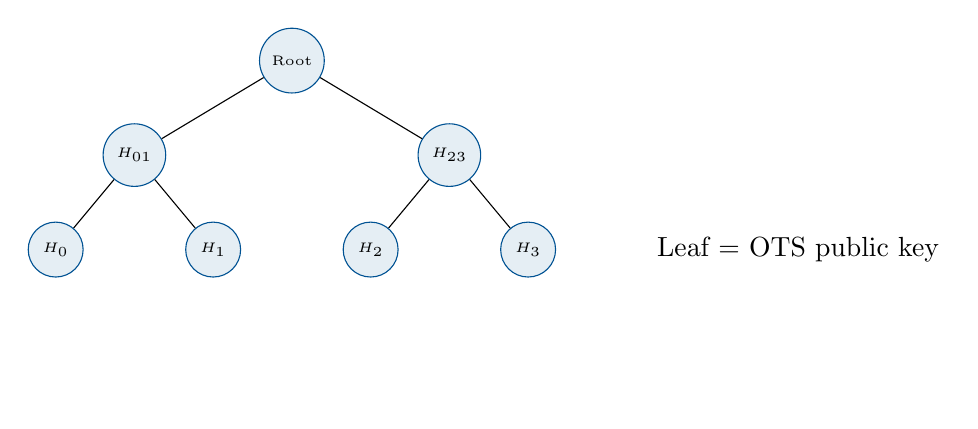
\begin{tikzpicture}[
    level distance=1.2cm,
    level 1/.style={sibling distance=4cm},
    level 2/.style={sibling distance=2cm},
    every node/.style={circle, draw=primaryblue, fill=primaryblue!10, minimum size=0.6cm, font=\tiny}
]
    \node {Root}
        child {node {$H_{01}$}
            child {node {$H_0$}}
            child {node {$H_1$}}
        }
        child {node {$H_{23}$}
            child {node {$H_2$}}
            child {node {$H_3$}}
        };
        
    \node[draw=none, fill=none, right=2cm] at (2.5, -2.4) {\normalsize Leaf = OTS public key};
\end{tikzpicture}
\end{center}

\section{Code-Based Cryptography}

Based on the difficulty of decoding random linear codes.

\subsection{McEliece Cryptosystem (1978)}

\begin{enumerate}[leftmargin=*, nosep]
    \item Generate a decodable code with generator matrix $G$
    \item Disguise it: $G' = SGP$ (scramble and permute)
    \item Public key: $G'$ \quad Private key: $S, G, P$
    \item Encrypt: $c = mG' + e$ (add errors)
    \item Decrypt: Use private key to decode
\end{enumerate}

\begin{warningbox}[Large Keys]
McEliece public keys are $\sim$1 MB at 128-bit security. This limits its use to specific applications.
\end{warningbox}

\section{Algorithm Family Comparison}

\begin{table}[h]
\centering
\caption{PQC Family Comparison}
\begin{tabular}{@{}lcccl@{}}
\toprule
\textbf{Family} & \textbf{Key Size} & \textbf{Speed} & \textbf{Maturity} & \textbf{Best For} \\
\midrule
Lattice & Small & Fast & Medium & General use \\
Hash-based & Small/Med & Slow & High & Long-term security \\
Code-based & Large & Fast & High & Key encapsulation \\
\bottomrule
\end{tabular}
\end{table}

% ============================================
% CHAPTER 4: NIST PQC STANDARDS
% ============================================
\chapter{NIST PQC Standards}

In August 2024, NIST released the first post-quantum cryptography standards after an 8-year evaluation process.

\section{Standardization Timeline}

\begin{center}
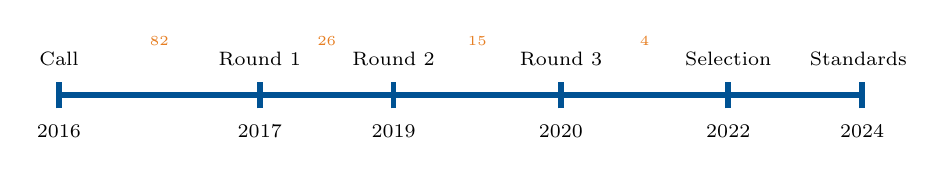
\begin{tikzpicture}[scale=0.85]
    % Timeline
    \draw[line width=2pt, primaryblue] (0,0) -- (12,0);
    
    % Events
    \foreach \x/\year/\event in {
        0/2016/Call,
        3/2017/Round 1,
        5/2019/Round 2,
        7.5/2020/Round 3,
        10/2022/Selection,
        12/2024/Standards
    } {
        \draw[primaryblue, line width=2pt] (\x,-0.2) -- (\x,0.2);
        \node[below, font=\scriptsize] at (\x,-0.3) {\year};
        \node[above, font=\scriptsize, align=center] at (\x,0.3) {\event};
    }
    
    % Submissions count
    \node[font=\tiny, accentorange] at (1.5, 0.8) {82};
    \node[font=\tiny, accentorange] at (4, 0.8) {26};
    \node[font=\tiny, accentorange] at (6.25, 0.8) {15};
    \node[font=\tiny, accentorange] at (8.75, 0.8) {4};
\end{tikzpicture}
\end{center}

\section{The Four Standardized Algorithms}

\begin{center}
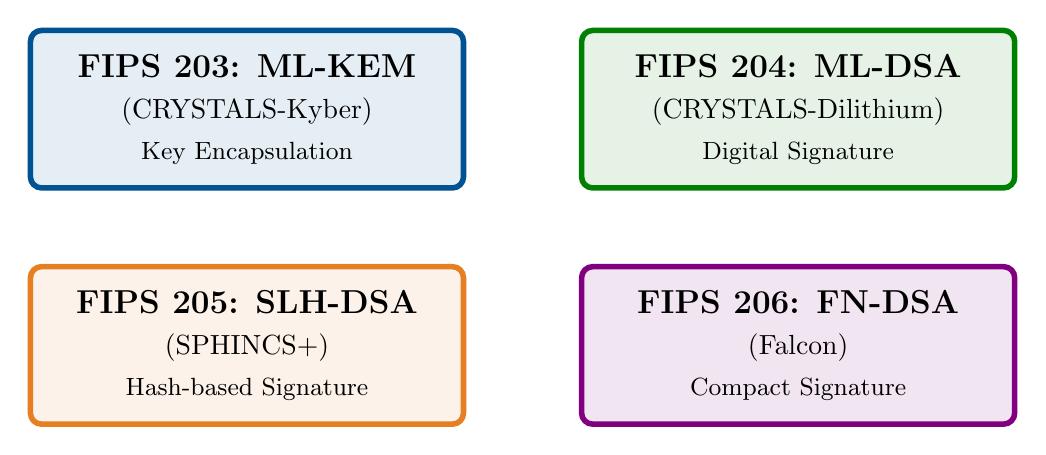
\begin{tikzpicture}[
    std/.style={rectangle, draw=#1, line width=2pt, fill=#1!10, 
                minimum width=5.5cm, minimum height=2cm, rounded corners, align=center}
]
    % KEM
    \node[std=primaryblue] (kyber) at (-3.5, 2) {
        \textbf{\large FIPS 203: ML-KEM}\\[0.1cm]
        (CRYSTALS-Kyber)\\[0.1cm]
        \small Key Encapsulation
    };
    
    % Signatures
    \node[std=secondarygreen] (dili) at (3.5, 2) {
        \textbf{\large FIPS 204: ML-DSA}\\[0.1cm]
        (CRYSTALS-Dilithium)\\[0.1cm]
        \small Digital Signature
    };
    
    \node[std=accentorange] (sphincs) at (-3.5, -1) {
        \textbf{\large FIPS 205: SLH-DSA}\\[0.1cm]
        (SPHINCS+)\\[0.1cm]
        \small Hash-based Signature
    };
    
    \node[std=quantumpurple] (falcon) at (3.5, -1) {
        \textbf{\large FIPS 206: FN-DSA}\\[0.1cm]
        (Falcon)\\[0.1cm]
        \small Compact Signature
    };
\end{tikzpicture}
\end{center}

\section{ML-KEM (Kyber)}

\textbf{Purpose:} Key Encapsulation Mechanism (establishes shared secrets)

\begin{table}[h]
\centering
\caption{ML-KEM Parameter Sets}
\begin{tabular}{@{}lcccc@{}}
\toprule
\textbf{Variant} & \textbf{Security} & \textbf{Public Key} & \textbf{Ciphertext} & \textbf{Shared Secret} \\
\midrule
ML-KEM-512 & Level 1 & 800 B & 768 B & 32 B \\
ML-KEM-768 & Level 3 & 1,184 B & 1,088 B & 32 B \\
ML-KEM-1024 & Level 5 & 1,568 B & 1,568 B & 32 B \\
\bottomrule
\end{tabular}
\end{table}

\subsection{How ML-KEM Works}

\begin{center}
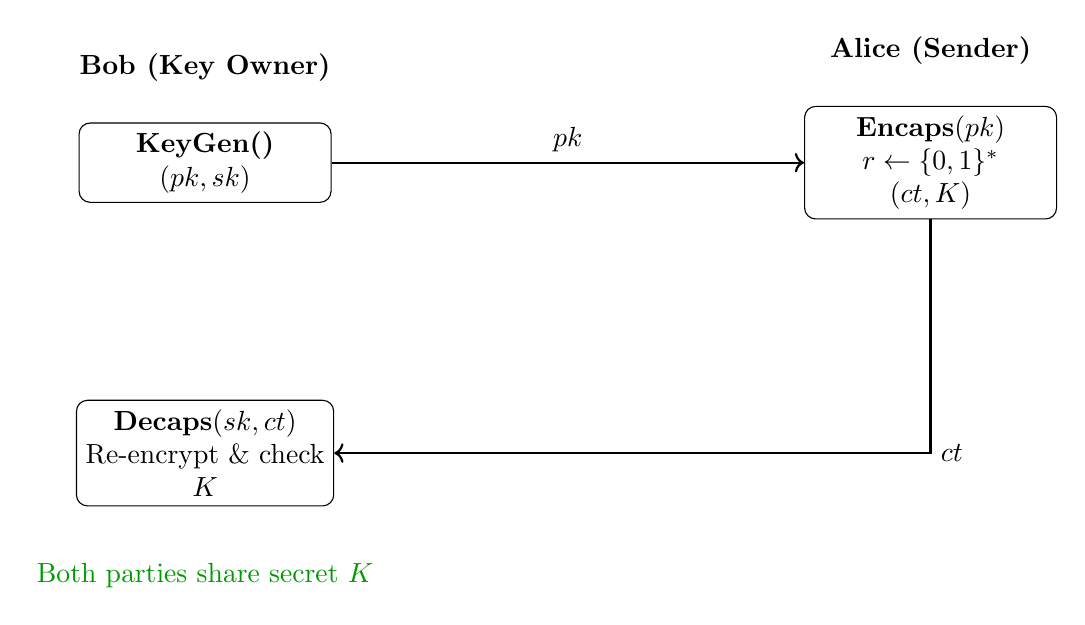
\begin{tikzpicture}[
    box/.style={draw, rounded corners, minimum width=3.2cm, minimum height=1cm, align=center},
    arrow/.style={->, thick}
]

% Bob side
\node[box] (keygen) {%
\textbf{KeyGen()}\\
$(pk, sk)$
};

% Alice side
\node[box, right=6cm of keygen] (encaps) {%
\textbf{Encaps}$(pk)$\\
$r \leftarrow \{0,1\}^*$\\
$(ct, K)$
};

\node[box, below=2.5cm of keygen] (decaps) {%
\textbf{Decaps}$(sk, ct)$\\
Re-encrypt \& check\\
$K$
};

% Arrows
\draw[arrow] (keygen.east) -- node[above] {$pk$} (encaps.west);
\draw[arrow] (encaps.south) |- node[right] {$ct$} (decaps.east);

% Labels
\node[above=0.4cm of keygen] {\textbf{Bob (Key Owner)}};
\node[above=0.4cm of encaps] {\textbf{Alice (Sender)}};

\node[below=0.6cm of decaps] {\textcolor{green!60!black}{Both parties share secret $K$}};

\end{tikzpicture}
\end{center}

\section{ML-DSA (Dilithium)}

\textbf{Purpose:} Digital signatures (authentication)

\begin{table}[h]
\centering
\caption{ML-DSA Parameter Sets}
\begin{tabular}{@{}lccccc@{}}
\toprule
\textbf{Variant} & \textbf{Security} & \textbf{Public Key} & \textbf{Private Key} & \textbf{Signature} \\
\midrule
ML-DSA-44 & Level 2 & 1,312 B & 2,560 B & 2,420 B \\
ML-DSA-65 & Level 3 & 1,952 B & 4,032 B & 3,309 B \\
ML-DSA-87 & Level 5 & 2,592 B & 4,896 B & 4,627 B \\
\bottomrule
\end{tabular}
\end{table}

\section{SLH-DSA (SPHINCS+)}

\textbf{Purpose:} Conservative hash-based signatures

\begin{infobox}[Why SPHINCS+?]
SPHINCS+ relies \textbf{only} on hash function security. If lattice problems are broken, SPHINCS+ remains secure. It's the ``backup plan.''
\end{infobox}

\textbf{Trade-off:} Small keys (32-64 bytes) but large signatures (8-50 KB).

\section{Comparison Summary}

\begin{table}[h]
\centering
\caption{NIST Standards Comparison (Level 3)}
\begin{tabular}{@{}lcccc@{}}
\toprule
\textbf{Algorithm} & \textbf{Type} & \textbf{Pub Key} & \textbf{Priv Key} & \textbf{Sig/CT} \\
\midrule
ML-KEM-768 & KEM & 1,184 B & 2,400 B & 1,088 B \\
ML-DSA-65 & Signature & 1,952 B & 4,032 B & 3,309 B \\
SLH-DSA-128f & Signature & 32 B & 64 B & 17,088 B \\
\bottomrule
\end{tabular}
\end{table}

\begin{keypoint}[Recommendation]
\textbf{For most applications:} Use ML-KEM for key exchange and ML-DSA for signatures. Use SLH-DSA when conservative security assumptions are critical.
\end{keypoint}

% ============================================
% CHAPTER 5: GPU ARCHITECTURE & CUDA
% ============================================
\chapter{GPU Architecture and CUDA}

\section{GPU vs CPU Architecture}

GPUs and CPUs are designed for fundamentally different tasks:

\begin{center}
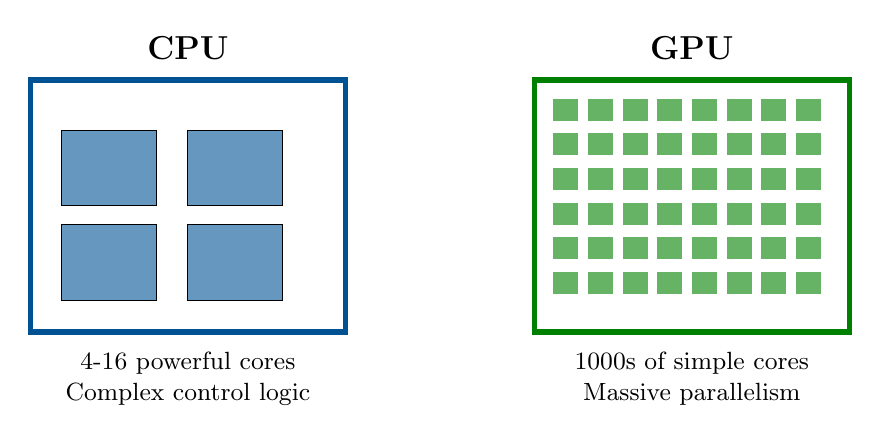
\begin{tikzpicture}[scale=0.8]
    % CPU
    \node[font=\bfseries\large] at (-4, 4) {CPU};
    \draw[line width=2pt, primaryblue] (-6.5, -0.5) rectangle (-1.5, 3.5);
    
    % CPU cores (few, large)
    \foreach \x in {0,1} {
        \foreach \y in {0,1} {
            \draw[fill=primaryblue!60] (-6+\x*2, 0+\y*1.5) rectangle (-4.5+\x*2, 1.2+\y*1.5);
        }
    }
    \node[font=\small] at (-4, -1) {4-16 powerful cores};
    \node[font=\small] at (-4, -1.5) {Complex control logic};
    
    % GPU
    \node[font=\bfseries\large] at (4, 4) {GPU};
    \draw[line width=2pt, secondarygreen] (1.5, -0.5) rectangle (6.5, 3.5);
    
    % GPU cores (many, small)
    \foreach \x in {0,...,7} {
        \foreach \y in {0,...,5} {
            \fill[secondarygreen!60] (1.8+\x*0.55, 0.1+\y*0.55) rectangle (2.2+\x*0.55, 0.45+\y*0.55);
        }
    }
    \node[font=\small] at (4, -1) {1000s of simple cores};
    \node[font=\small] at (4, -1.5) {Massive parallelism};
\end{tikzpicture}
\end{center}

\begin{table}[h]
\centering
\caption{CPU vs GPU Characteristics}
\begin{tabular}{@{}lcc@{}}
\toprule
\textbf{Feature} & \textbf{CPU} & \textbf{GPU} \\
\midrule
Core count & 4-64 & 1,000-16,000 \\
Clock speed & 3-5 GHz & 1-2 GHz \\
Cache per core & Large (MB) & Small (KB) \\
Best for & Sequential tasks & Parallel tasks \\
Control flow & Complex branching & Simple SIMD \\
\bottomrule
\end{tabular}
\end{table}

\section{CUDA Programming Model}

\textbf{CUDA} (Compute Unified Device Architecture) is NVIDIA's parallel computing platform.

\subsection{Key Concepts}

\begin{center}
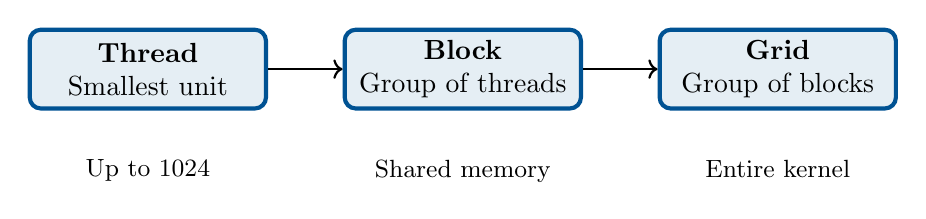
\begin{tikzpicture}[
    concept/.style={rectangle, draw=primaryblue, line width=1.5pt, fill=primaryblue!10, 
                    rounded corners, minimum width=3cm, minimum height=1cm, align=center}
]
    \node[concept] (thread) at (0, 0) {\textbf{Thread}\\Smallest unit};
    \node[concept] (block) at (4, 0) {\textbf{Block}\\Group of threads};
    \node[concept] (grid) at (8, 0) {\textbf{Grid}\\Group of blocks};
    
    \draw[->, thick] (thread) -- (block);
    \draw[->, thick] (block) -- (grid);
    
    \node[below=0.5cm of thread, font=\small] {Up to 1024};
    \node[below=0.5cm of block, font=\small] {Shared memory};
    \node[below=0.5cm of grid, font=\small] {Entire kernel};
\end{tikzpicture}
\end{center}

\subsection{Thread Hierarchy}

\begin{center}
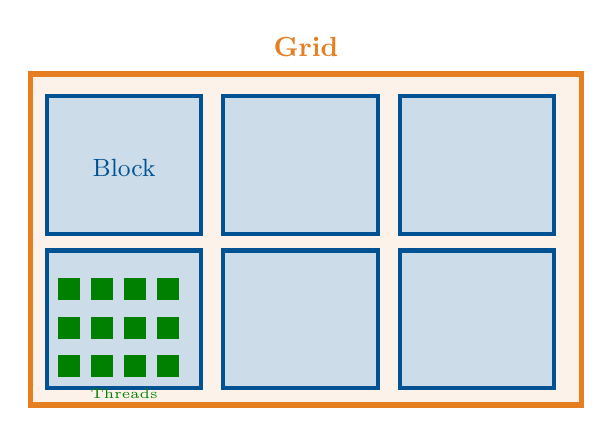
\begin{tikzpicture}[scale=0.7]
    % Grid
    \draw[line width=2pt, accentorange, fill=accentorange!10] (0,0) rectangle (10, 6);
    \node[font=\bfseries, accentorange] at (5, 6.5) {Grid};
    
    % Blocks
    \foreach \bx in {0,1,2} {
        \foreach \by in {0,1} {
            \draw[line width=1.5pt, primaryblue, fill=primaryblue!20] 
                (0.3+\bx*3.2, 0.3+\by*2.8) rectangle (3.1+\bx*3.2, 2.8+\by*2.8);
        }
    }
    \node[font=\small, primaryblue] at (1.7, 4.3) {Block};
    
    % Threads in one block
    \foreach \tx in {0,...,3} {
        \foreach \ty in {0,...,2} {
            \fill[secondarygreen] (0.5+\tx*0.6, 0.5+\ty*0.7) rectangle (0.9+\tx*0.6, 0.9+\ty*0.7);
        }
    }
    \node[font=\tiny, secondarygreen] at (1.7, 0.2) {Threads};
\end{tikzpicture}
\end{center}

\section{CUDA Memory Model}

\begin{center}
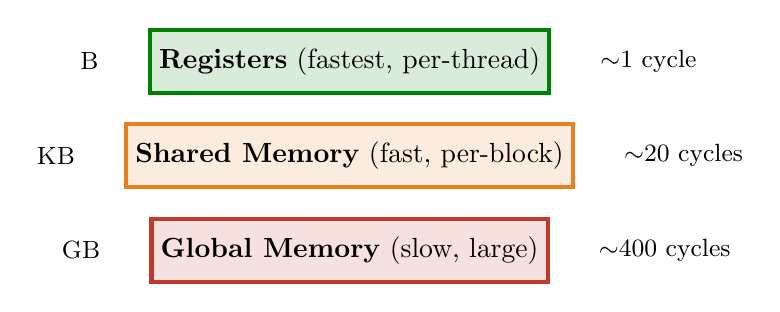
\begin{tikzpicture}[
    mem/.style={rectangle, draw=#1, line width=1.5pt, fill=#1!15, 
                minimum width=4cm, minimum height=0.8cm, align=center}
]
    \node[mem=hardwarered] (global) at (0, 0) {\textbf{Global Memory} (slow, large)};
    \node[mem=accentorange] (shared) at (0, 1.2) {\textbf{Shared Memory} (fast, per-block)};
    \node[mem=secondarygreen] (reg) at (0, 2.4) {\textbf{Registers} (fastest, per-thread)};
    
    % Latency labels
    \node[right=0.5cm of global, font=\small] {$\sim$400 cycles};
    \node[right=0.5cm of shared, font=\small] {$\sim$20 cycles};
    \node[right=0.5cm of reg, font=\small] {$\sim$1 cycle};
    
    % Size labels
    \node[left=0.5cm of global, font=\small] {GB};
    \node[left=0.5cm of shared, font=\small] {KB};
    \node[left=0.5cm of reg, font=\small] {B};
\end{tikzpicture}
\end{center}

\section{CUDA Kernel Example}

A \textbf{kernel} is a function that runs on the GPU:

\begin{tcolorbox}[colback=codebg, colframe=primaryblue, title=Vector Addition Kernel]
\begin{lstlisting}[language=C, basicstyle=\small\ttfamily, keywordstyle=\color{primaryblue}]
__global__ void vectorAdd(float *a, float *b, 
                          float *c, int n) {
    int i = blockIdx.x * blockDim.x + threadIdx.x;
    if (i < n) {
        c[i] = a[i] + b[i];
    }
}

// Launch: vectorAdd<<<numBlocks, blockSize>>>(...)
\end{lstlisting}
\end{tcolorbox}

\subsection{Execution Flow}

\begin{center}
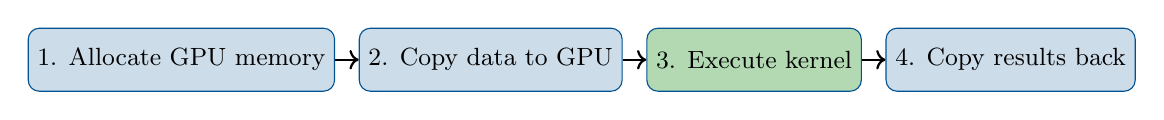
\begin{tikzpicture}[
    flowstep/.style={rectangle, draw=primaryblue, rounded corners, minimum width=2.5cm, 
                 minimum height=0.8cm, align=center, font=\small},
    node distance=0.3cm
]
    \node[flowstep, fill=primaryblue!20] (alloc) {1. Allocate GPU memory};
    \node[flowstep, fill=primaryblue!20, right=of alloc] (copy1) {2. Copy data to GPU};
    \node[flowstep, fill=secondarygreen!30, right=of copy1] (kernel) {3. Execute kernel};
    \node[flowstep, fill=primaryblue!20, right=of kernel] (copy2) {4. Copy results back};
    
    \draw[->, thick] (alloc) -- (copy1);
    \draw[->, thick] (copy1) -- (kernel);
    \draw[->, thick] (kernel) -- (copy2);
\end{tikzpicture}
\end{center}

\section{Performance Considerations}

\begin{keypoint}[Optimization Tips]
\begin{enumerate}[leftmargin=*, nosep]
    \item \textbf{Maximize parallelism:} Launch thousands of threads
    \item \textbf{Minimize memory transfers:} CPU$\leftrightarrow$GPU is slow
    \item \textbf{Use shared memory:} Cache frequently accessed data
    \item \textbf{Coalesce memory access:} Adjacent threads access adjacent memory
    \item \textbf{Avoid branch divergence:} Threads in a warp should follow same path
\end{enumerate}
\end{keypoint}

\section{CUDA Libraries for Compression}

NVIDIA provides optimized libraries:

\begin{table}[h]
\centering
\caption{NVIDIA Compression Libraries}
\begin{tabular}{@{}llc@{}}
\toprule
\textbf{Library} & \textbf{Algorithms} & \textbf{Throughput} \\
\midrule
nvCOMP & LZ4, Snappy, DEFLATE, zstd & Up to 500 GB/s \\
cuBLAS & Linear algebra (for transforms) & Optimized \\
cuFFT & FFT (for frequency domain) & Optimized \\
\bottomrule
\end{tabular}
\end{table}

\begin{infobox}[nvCOMP Performance]
nvCOMP can achieve \textbf{150$\times$} speedup over CPU implementations for batch compression of small blocks.
\end{infobox}

% ============================================
% CHAPTER 6: OpenCL & Cross-Platform
% ============================================

\chapter{OpenCL and Cross-Platform Computing}

\section{Introduction to OpenCL}

\textbf{OpenCL (Open Computing Language)} is an open standard for parallel programming across heterogeneous platforms---CPUs, GPUs, FPGAs, and DSPs from different vendors.

\begin{keypoint}
OpenCL provides \textbf{vendor-neutral} parallel computing, enabling the same code to run on AMD, Intel, NVIDIA, and ARM devices.
\end{keypoint}

\subsection{Platform Model}

\begin{center}
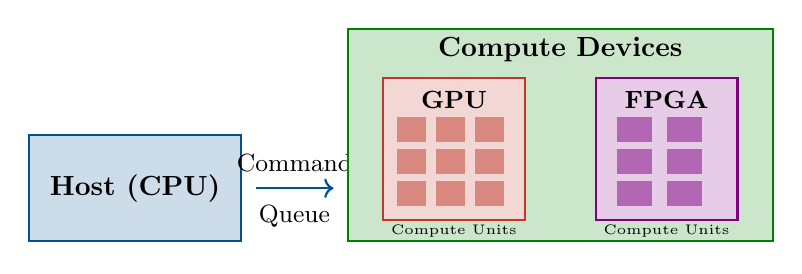
\begin{tikzpicture}[scale=0.9]
    % Host
    \fill[primaryblue!20] (0,0) rectangle (3,1.5);
    \draw[primaryblue, thick] (0,0) rectangle (3,1.5);
    \node at (1.5,0.75) {\textbf{Host (CPU)}};
    
    % Arrow
    \draw[->, thick, primaryblue] (3.2,0.75) -- (4.3,0.75);
    \node[above] at (3.75,0.85) {\small Command};
    \node[below] at (3.75,0.65) {\small Queue};
    
    % Compute Devices
    \fill[secondarygreen!20] (4.5,0) rectangle (10.5,3);
    \draw[secondarygreen, thick] (4.5,0) rectangle (10.5,3);
    \node at (7.5,2.7) {\textbf{Compute Devices}};
    
    % Device 1 - GPU
    \fill[hardwarered!20] (5,0.3) rectangle (7,2.3);
    \draw[hardwarered, thick] (5,0.3) rectangle (7,2.3);
    \node at (6,2) {\small \textbf{GPU}};
    \foreach \i in {0,1,2} {
        \foreach \j in {0,1,2} {
            \fill[hardwarered!60] (5.2+\i*0.55,0.5+\j*0.45) rectangle (5.6+\i*0.55,0.85+\j*0.45);
        }
    }
    \node at (6,0.15) {\tiny Compute Units};
    
    % Device 2 - FPGA
    \fill[quantumpurple!20] (8,0.3) rectangle (10,2.3);
    \draw[quantumpurple, thick] (8,0.3) rectangle (10,2.3);
    \node at (9,2) {\small \textbf{FPGA}};
    \foreach \i in {0,1} {
        \foreach \j in {0,1,2} {
            \fill[quantumpurple!60] (8.3+\i*0.7,0.5+\j*0.45) rectangle (8.8+\i*0.7,0.85+\j*0.45);
        }
    }
    \node at (9,0.15) {\tiny Compute Units};
\end{tikzpicture}
\end{center}

\subsection{OpenCL Architecture Layers}

\begin{enumerate}[leftmargin=*]
    \item \textbf{Platform Model}: Host + compute devices with compute units and processing elements
    \item \textbf{Execution Model}: Kernels executed by work-items organized in work-groups
    \item \textbf{Memory Model}: Global, local, constant, and private memory regions
    \item \textbf{Programming Model}: Data-parallel and task-parallel execution
\end{enumerate}

\section{Memory Model}

OpenCL defines four memory regions with different scope and performance characteristics:

\begin{center}
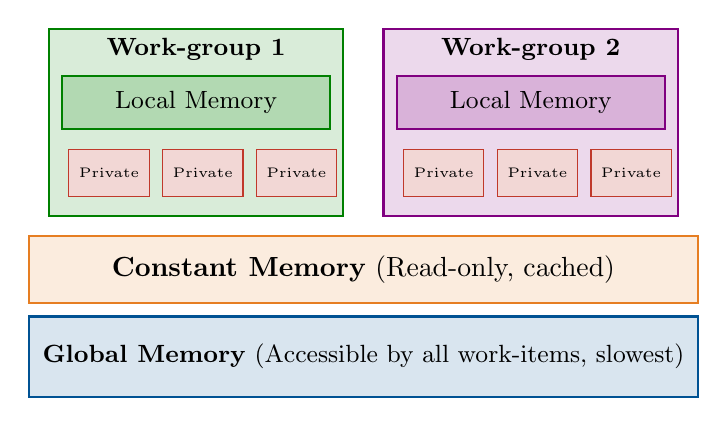
\begin{tikzpicture}[scale=0.85]
    % Global Memory
    \fill[primaryblue!15] (0,0) rectangle (10,1.2);
    \draw[primaryblue, thick] (0,0) rectangle (10,1.2);
    \node[font=\small] at (5,0.6) {\textbf{Global Memory} (Accessible by all work-items, slowest)};
    
    % Constant Memory
    \fill[accentorange!15] (0,1.4) rectangle (10,2.4);
    \draw[accentorange, thick] (0,1.4) rectangle (10,2.4);
    \node at (5,1.9) {\textbf{Constant Memory} (Read-only, cached)};
    
    % Work-group 1
    \fill[secondarygreen!15] (0.3,2.7) rectangle (4.7,5.5);
    \draw[secondarygreen, thick] (0.3,2.7) rectangle (4.7,5.5);
    \node at (2.5,5.2) {\small \textbf{Work-group 1}};
    
    % Local memory 1
    \fill[secondarygreen!30] (0.5,4) rectangle (4.5,4.8);
    \draw[secondarygreen, thick] (0.5,4) rectangle (4.5,4.8);
    \node at (2.5,4.4) {\small Local Memory};
    
    % Private memories 1
    \fill[hardwarered!20] (0.6,3) rectangle (1.8,3.7);
    \draw[hardwarered] (0.6,3) rectangle (1.8,3.7);
    \node at (1.2,3.35) {\tiny Private};
    
    \fill[hardwarered!20] (2,3) rectangle (3.2,3.7);
    \draw[hardwarered] (2,3) rectangle (3.2,3.7);
    \node at (2.6,3.35) {\tiny Private};
    
    \fill[hardwarered!20] (3.4,3) rectangle (4.6,3.7);
    \draw[hardwarered] (3.4,3) rectangle (4.6,3.7);
    \node at (4,3.35) {\tiny Private};
    
    % Work-group 2
    \fill[quantumpurple!15] (5.3,2.7) rectangle (9.7,5.5);
    \draw[quantumpurple, thick] (5.3,2.7) rectangle (9.7,5.5);
    \node at (7.5,5.2) {\small \textbf{Work-group 2}};
    
    % Local memory 2
    \fill[quantumpurple!30] (5.5,4) rectangle (9.5,4.8);
    \draw[quantumpurple, thick] (5.5,4) rectangle (9.5,4.8);
    \node at (7.5,4.4) {\small Local Memory};
    
    % Private memories 2
    \fill[hardwarered!20] (5.6,3) rectangle (6.8,3.7);
    \draw[hardwarered] (5.6,3) rectangle (6.8,3.7);
    \node at (6.2,3.35) {\tiny Private};
    
    \fill[hardwarered!20] (7,3) rectangle (8.2,3.7);
    \draw[hardwarered] (7,3) rectangle (8.2,3.7);
    \node at (7.6,3.35) {\tiny Private};
    
    \fill[hardwarered!20] (8.4,3) rectangle (9.6,3.7);
    \draw[hardwarered] (8.4,3) rectangle (9.6,3.7);
    \node at (9,3.35) {\tiny Private};
\end{tikzpicture}
\end{center}

\begin{table}[h]
\centering
\caption{OpenCL Memory Regions}
\begin{tabular}{@{}llll@{}}
\toprule
\textbf{Memory} & \textbf{Scope} & \textbf{Speed} & \textbf{Size} \\
\midrule
Global & All work-items & Slow & Large (GBs) \\
Constant & All (read-only) & Fast (cached) & Limited (64KB) \\
Local & Work-group & Fast & Small (48KB) \\
Private & Single work-item & Fastest & Very small \\
\bottomrule
\end{tabular}
\end{table}

\section{OpenCL Kernel Programming}

\subsection{Kernel Syntax}

OpenCL kernels are written in OpenCL C, a subset of C99 with extensions:

\begin{lstlisting}[language=C, caption=OpenCL Vector Addition Kernel]
__kernel void vector_add(
    __global const float* A,
    __global const float* B,
    __global float* C,
    const int N)
{
    int gid = get_global_id(0);
    if (gid < N) {
        C[gid] = A[gid] + B[gid];
    }
}
\end{lstlisting}

\subsection{Key OpenCL Functions}

\begin{table}[h]
\centering
\begin{tabular}{@{}ll@{}}
\toprule
\textbf{Function} & \textbf{Purpose} \\
\midrule
\texttt{get\_global\_id(dim)} & Global work-item ID \\
\texttt{get\_local\_id(dim)} & Local ID within work-group \\
\texttt{get\_group\_id(dim)} & Work-group ID \\
\texttt{get\_global\_size(dim)} & Total number of work-items \\
\texttt{get\_local\_size(dim)} & Work-group size \\
\texttt{barrier()} & Synchronization within work-group \\
\bottomrule
\end{tabular}
\end{table}

\section{CUDA vs OpenCL Comparison}

\begin{table}[h]
\centering
\caption{CUDA vs OpenCL Feature Comparison}
\begin{tabular}{@{}lll@{}}
\toprule
\textbf{Aspect} & \textbf{CUDA} & \textbf{OpenCL} \\
\midrule
Vendor & NVIDIA only & Cross-platform \\
Performance & Highly optimized & Vendor-dependent \\
Terminology & Threads, Blocks, Grids & Work-items, Work-groups, NDRange \\
Memory & Shared, Global & Local, Global \\
Ecosystem & Mature libraries & Broader hardware support \\
Learning Curve & Easier & More complex \\
\bottomrule
\end{tabular}
\end{table}

\begin{warningbox}
While OpenCL offers portability, \textbf{CUDA typically achieves 10-30\% better performance} on NVIDIA hardware due to vendor-specific optimizations.
\end{warningbox}

% ============================================
% CHAPTER 7: FPGA Architecture
% ============================================

\chapter{FPGA Architecture and Programming}

\section{Introduction to FPGAs}

\textbf{Field-Programmable Gate Arrays (FPGAs)} are integrated circuits that can be configured after manufacturing to implement custom digital logic.

\begin{keypoint}
Unlike GPUs that execute instructions, FPGAs implement algorithms \textbf{directly in hardware}, achieving extreme parallelism and energy efficiency.
\end{keypoint}

\section{FPGA Architecture}

\subsection{Core Components}

\begin{center}
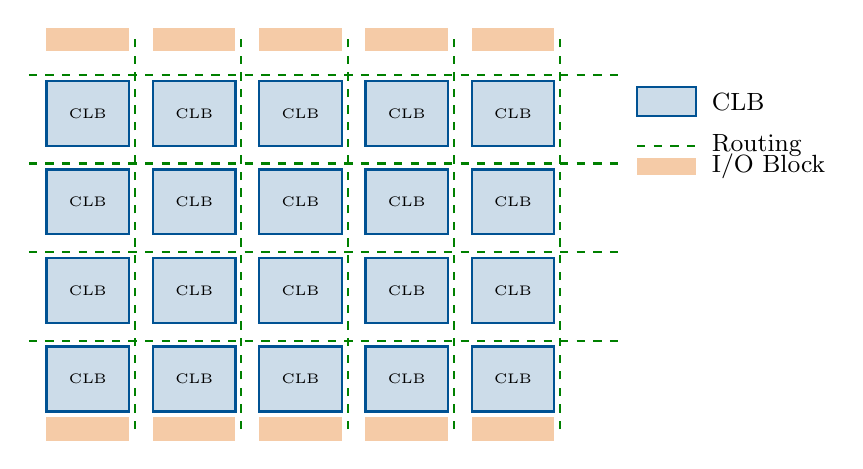
\begin{tikzpicture}[scale=0.75]
    % Grid of CLBs
    \foreach \i in {0,1,2,3,4} {
        \foreach \j in {0,1,2,3} {
            \fill[primaryblue!20] (\i*1.8,\j*1.5) rectangle (\i*1.8+1.4,\j*1.5+1.1);
            \draw[primaryblue, thick] (\i*1.8,\j*1.5) rectangle (\i*1.8+1.4,\j*1.5+1.1);
            \node at (\i*1.8+0.7,\j*1.5+0.55) {\tiny CLB};
        }
    }
    
    % Routing channels (horizontal)
    \foreach \j in {0,1,2,3} {
        \draw[secondarygreen, thick, dashed] (-0.3,\j*1.5+1.2) -- (9.7,\j*1.5+1.2);
    }
    
    % Routing channels (vertical)
    \foreach \i in {0,1,2,3,4} {
        \draw[secondarygreen, thick, dashed] (\i*1.8+1.5,-.3) -- (\i*1.8+1.5,6.3);
    }
    
    % I/O blocks on edges
    \foreach \i in {0,1,2,3,4} {
        \fill[accentorange!40] (\i*1.8,-0.5) rectangle (\i*1.8+1.4,-0.1);
        \fill[accentorange!40] (\i*1.8,6.1) rectangle (\i*1.8+1.4,6.5);
    }
    
    % Legend
    \fill[primaryblue!20] (10,5) rectangle (11,5.5);
    \draw[primaryblue, thick] (10,5) rectangle (11,5.5);
    \node[right] at (11.1,5.25) {\small CLB};
    
    \draw[secondarygreen, thick, dashed] (10,4.5) -- (11,4.5);
    \node[right] at (11.1,4.5) {\small Routing};
    
    \fill[accentorange!40] (10,4) rectangle (11,4.3);
    \node[right] at (11.1,4.15) {\small I/O Block};
\end{tikzpicture}
\end{center}

\begin{itemize}[leftmargin=*]
    \item \textbf{Configurable Logic Blocks (CLBs)}: Contain LUTs, flip-flops, and multiplexers
    \item \textbf{Programmable Interconnect}: Routing matrix connecting CLBs
    \item \textbf{I/O Blocks}: Interface with external devices
    \item \textbf{Block RAM (BRAM)}: Dedicated memory blocks
    \item \textbf{DSP Slices}: Hardened multiply-accumulate units
\end{itemize}

\subsection{Look-Up Table (LUT) Structure}

A LUT implements any boolean function by storing the truth table in memory:

\begin{center}
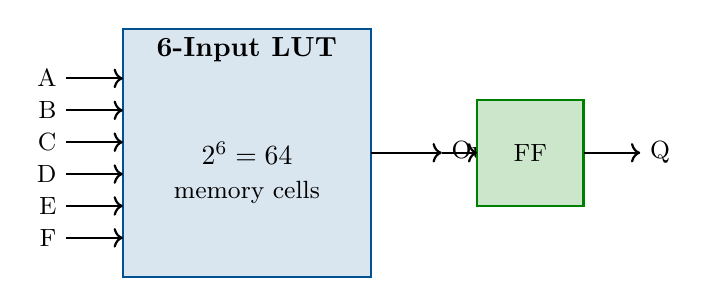
\begin{tikzpicture}[scale=0.9]
    % LUT Box
    \fill[primaryblue!15] (0,0) rectangle (3.5,3.5);
    \draw[primaryblue, thick] (0,0) rectangle (3.5,3.5);
    \node at (1.75,3.2) {\textbf{6-Input LUT}};
    
    % Inputs
    \foreach \i/\label in {0/A,1/B,2/C,3/D,4/E,5/F} {
        \draw[thick, ->] (-0.8,2.8-\i*0.45) -- (0,2.8-\i*0.45);
        \node[left] at (-0.8,2.8-\i*0.45) {\small \label};
    }
    
    % Memory cells representation
    \node at (1.75,1.75) {$2^6 = 64$};
    \node at (1.75,1.2) {\small memory cells};
    
    % Output
    \draw[thick, ->] (3.5,1.75) -- (4.5,1.75);
    \node[right] at (4.5,1.75) {\small Output};
    
    % Flip-flop
    \fill[secondarygreen!20] (5,1) rectangle (6.5,2.5);
    \draw[secondarygreen, thick] (5,1) rectangle (6.5,2.5);
    \node at (5.75,1.75) {\small FF};
    \draw[thick, ->] (4.5,1.75) -- (5,1.75);
    \draw[thick, ->] (6.5,1.75) -- (7.3,1.75);
    \node[right] at (7.3,1.75) {\small Q};
\end{tikzpicture}
\end{center}

\section{FPGA vs GPU vs CPU}

\begin{table}[h]
\centering
\caption{Hardware Platform Comparison}
\begin{tabular}{@{}llll@{}}
\toprule
\textbf{Metric} & \textbf{CPU} & \textbf{GPU} & \textbf{FPGA} \\
\midrule
Parallelism & Low (8-64 cores) & High (thousands) & Extreme (custom) \\
Flexibility & Very high & High & Medium \\
Power Efficiency & Low & Medium & High \\
Latency & Medium & High & Very low \\
Development Time & Fast & Medium & Slow \\
Throughput & Low & Very high & High \\
\bottomrule
\end{tabular}
\end{table}

\section{FPGA Programming Methods}

\subsection{Traditional HDL Flow}

\begin{center}
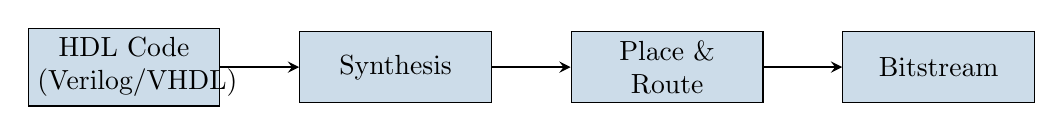
\begin{tikzpicture}[node distance=1.5cm, auto,
    block/.style={rectangle, draw, fill=primaryblue!20, text width=2.2cm, text centered, minimum height=0.9cm},
    arrow/.style={thick, ->, >=stealth}]
    
    \node[block] (hdl) {HDL Code\\(Verilog/VHDL)};
    \node[block, right=1cm of hdl] (synth) {Synthesis};
    \node[block, right=1cm of synth] (pnr) {Place \& Route};
    \node[block, right=1cm of pnr] (bit) {Bitstream};
    
    \draw[arrow] (hdl) -- (synth);
    \draw[arrow] (synth) -- (pnr);
    \draw[arrow] (pnr) -- (bit);
\end{tikzpicture}
\end{center}

\subsection{High-Level Synthesis (HLS)}

Modern FPGAs support \textbf{High-Level Synthesis}, allowing C/C++/OpenCL code to be compiled to hardware:

\begin{lstlisting}[language=C, caption=HLS Example - Matrix Multiply]
void matmul(float A[N][K], float B[K][M], float C[N][M]) {
    #pragma HLS INTERFACE m_axi port=A
    #pragma HLS INTERFACE m_axi port=B
    #pragma HLS INTERFACE m_axi port=C
    
    for (int i = 0; i < N; i++) {
        for (int j = 0; j < M; j++) {
            #pragma HLS PIPELINE II=1
            float sum = 0;
            for (int k = 0; k < K; k++) {
                sum += A[i][k] * B[k][j];
            }
            C[i][j] = sum;
        }
    }
}
\end{lstlisting}

\begin{infobox}[HLS Pragmas]
HLS pragmas guide the compiler to optimize for:
\begin{itemize}
    \item \texttt{PIPELINE}: Enable pipelined execution
    \item \texttt{UNROLL}: Replicate loop iterations in hardware
    \item \texttt{ARRAY\_PARTITION}: Distribute arrays across BRAMs
\end{itemize}
\end{infobox}

\section{Major FPGA Vendors}

\begin{table}[h]
\centering
\begin{tabular}{@{}lll@{}}
\toprule
\textbf{Vendor} & \textbf{Product Lines} & \textbf{Tools} \\
\midrule
AMD/Xilinx & Versal, UltraScale+, Artix & Vivado, Vitis \\
Intel/Altera & Agilex, Stratix, Cyclone & Quartus Prime \\
Lattice & CrossLink-NX, ECP5 & Radiant, Diamond \\
Microchip & PolarFire, SmartFusion & Libero SoC \\
\bottomrule
\end{tabular}
\end{table}

% ============================================
% CHAPTER 8: Hardware-Accelerated Compression
% ============================================

\chapter{Hardware-Accelerated Compression}

\section{Why Hardware Acceleration?}

Data compression is computationally intensive. Hardware acceleration addresses:

\begin{enumerate}[leftmargin=*]
    \item \textbf{Throughput}: Process data faster than CPU alone
    \item \textbf{Latency}: Reduce compression/decompression time
    \item \textbf{Energy}: Lower power consumption per operation
    \item \textbf{CPU Offloading}: Free CPU for other tasks
\end{enumerate}

\begin{center}
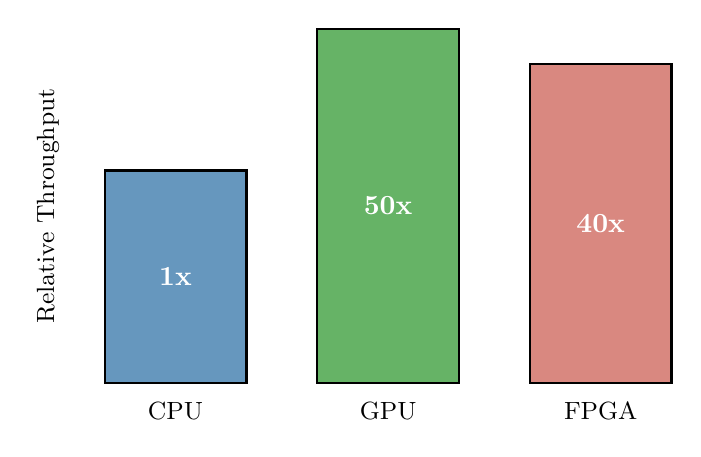
\begin{tikzpicture}[scale=0.9]
    % CPU bar
    \fill[primaryblue!60] (0,0) rectangle (2,3);
    \draw[thick] (0,0) rectangle (2,3);
    \node at (1,-0.4) {\small CPU};
    \node[white] at (1,1.5) {\textbf{1x}};
    
    % GPU bar
    \fill[secondarygreen!60] (3,0) rectangle (5,5);
    \draw[thick] (3,0) rectangle (5,5);
    \node at (4,-0.4) {\small GPU};
    \node[white] at (4,2.5) {\textbf{50x}};
    
    % FPGA bar
    \fill[hardwarered!60] (6,0) rectangle (8,4.5);
    \draw[thick] (6,0) rectangle (8,4.5);
    \node at (7,-0.4) {\small FPGA};
    \node[white] at (7,2.25) {\textbf{40x}};
    
    % Y-axis label
    \node[rotate=90] at (-0.8,2.5) {\small Relative Throughput};
\end{tikzpicture}
\end{center}

\section{GPU Compression Techniques}

\subsection{Parallel LZ77}

Traditional LZ77 is sequential (each match depends on previous output). GPU-optimized approaches:

\begin{itemize}[leftmargin=*]
    \item \textbf{Block-parallel}: Divide input into independent blocks
    \item \textbf{Hash-based matching}: Parallel hash table lookups
    \item \textbf{Batch processing}: Compress multiple streams simultaneously
\end{itemize}

\begin{center}
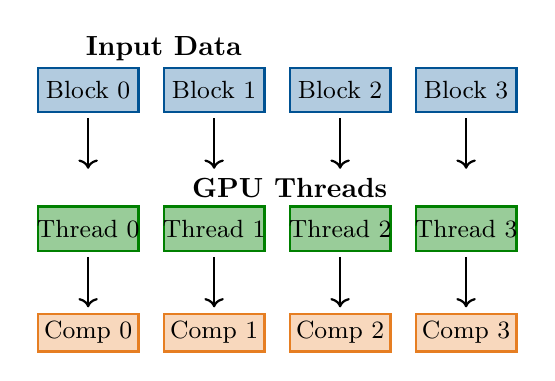
\begin{tikzpicture}[scale=0.8]
    % Input data blocks
    \node at (2,4.5) {\textbf{Input Data}};
    \foreach \i in {0,1,2,3} {
        \fill[primaryblue!30] (\i*2,3.5) rectangle (\i*2+1.6,4.2);
        \draw[primaryblue, thick] (\i*2,3.5) rectangle (\i*2+1.6,4.2);
        \node at (\i*2+0.8,3.85) {\small Block \i};
    }
    
    % Arrows
    \foreach \i in {0,1,2,3} {
        \draw[->, thick] (\i*2+0.8,3.4) -- (\i*2+0.8,2.6);
    }
    
    % GPU cores
    \node at (4,2.3) {\textbf{GPU Threads}};
    \foreach \i in {0,1,2,3} {
        \fill[secondarygreen!40] (\i*2,1.3) rectangle (\i*2+1.6,2);
        \draw[secondarygreen, thick] (\i*2,1.3) rectangle (\i*2+1.6,2);
        \node at (\i*2+0.8,1.65) {\small Thread \i};
    }
    
    % Arrows
    \foreach \i in {0,1,2,3} {
        \draw[->, thick] (\i*2+0.8,1.2) -- (\i*2+0.8,0.4);
    }
    
    % Output
    \foreach \i in {0,1,2,3} {
        \fill[accentorange!30] (\i*2,-0.3) rectangle (\i*2+1.6,0.3);
        \draw[accentorange, thick] (\i*2,-0.3) rectangle (\i*2+1.6,0.3);
        \node at (\i*2+0.8,0) {\small Comp \i};
    }
\end{tikzpicture}
\end{center}

\subsection{Parallel Huffman Coding}

\begin{enumerate}[leftmargin=*]
    \item \textbf{Histogram}: Parallel frequency counting (atomic operations)
    \item \textbf{Tree Building}: Sequential on CPU (small overhead)
    \item \textbf{Encoding}: Parallel symbol-to-code mapping
    \item \textbf{Bit Packing}: Parallel with careful synchronization
\end{enumerate}

\section{FPGA Compression Implementations}

FPGAs excel at compression due to:

\begin{keypoint}
FPGAs implement compression as \textbf{streaming pipelines}---data flows through dedicated hardware stages with single-cycle latency per stage.
\end{keypoint}

\subsection{Streaming LZ77 Architecture}

\begin{center}
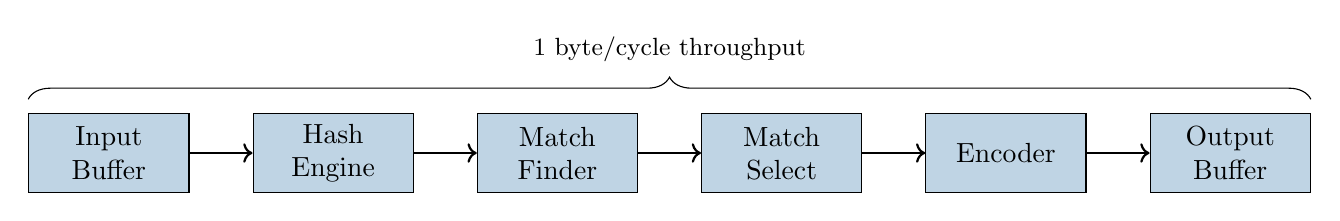
\begin{tikzpicture}[scale=0.85, node distance=0.8cm,
    stage/.style={rectangle, draw, fill=primaryblue!25, minimum width=2cm, minimum height=1cm, text width=1.8cm, align=center}]
    
    \node[stage] (input) {Input Buffer};
    \node[stage, right=of input] (hash) {Hash Engine};
    \node[stage, right=of hash] (match) {Match Finder};
    \node[stage, right=of match] (select) {Match Select};
    \node[stage, right=of select] (encode) {Encoder};
    \node[stage, right=of encode] (output) {Output Buffer};
    
    \draw[->, thick] (input) -- (hash);
    \draw[->, thick] (hash) -- (match);
    \draw[->, thick] (match) -- (select);
    \draw[->, thick] (select) -- (encode);
    \draw[->, thick] (encode) -- (output);
    
    % Pipeline annotation
    \draw[decorate, decoration={brace, amplitude=8pt, raise=5pt}] 
        (input.north west) -- (output.north east)
        node[midway, above=15pt] {\small 1 byte/cycle throughput};
\end{tikzpicture}
\end{center}

\subsection{Commercial FPGA Compression IP}

\begin{table}[h]
\centering
\caption{FPGA Compression IP Cores}
\begin{tabular}{@{}llll@{}}
\toprule
\textbf{Vendor} & \textbf{Algorithm} & \textbf{Throughput} & \textbf{Ratio} \\
\midrule
AMD/Xilinx & GZIP/ZSTD & 8 GB/s & 2.5-3x \\
Intel & GZIP & 10 GB/s & 2.5x \\
Atomic Rules & ZSTD & 100 Gbps & 3x \\
Eideticom & LZ4/ZSTD & 64 GB/s & 2-3x \\
\bottomrule
\end{tabular}
\end{table}

\section{Hybrid CPU-GPU-FPGA Systems}

Modern systems combine accelerators for optimal performance:

\begin{center}
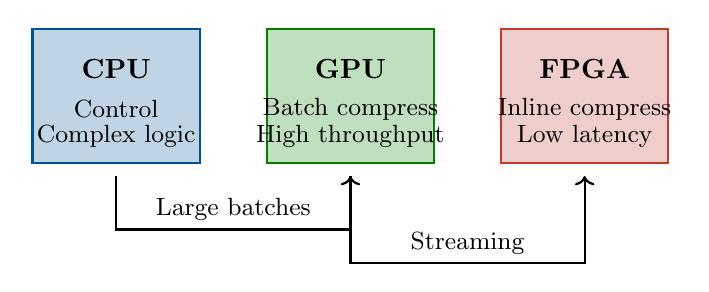
\begin{tikzpicture}[scale=0.85]
    % CPU
    \fill[primaryblue!25] (0,2) rectangle (2.5,4);
    \draw[primaryblue, thick] (0,2) rectangle (2.5,4);
    \node at (1.25,3.4) {\textbf{CPU}};
    \node at (1.25,2.8) {\small Control};
    \node at (1.25,2.4) {\small Complex logic};
    
    % GPU
    \fill[secondarygreen!25] (3.5,2) rectangle (6,4);
    \draw[secondarygreen, thick] (3.5,2) rectangle (6,4);
    \node at (4.75,3.4) {\textbf{GPU}};
    \node at (4.75,2.8) {\small Batch compress};
    \node at (4.75,2.4) {\small High throughput};
    
    % FPGA
    \fill[hardwarered!25] (7,2) rectangle (9.5,4);
    \draw[hardwarered, thick] (7,2) rectangle (9.5,4);
    \node at (8.25,3.4) {\textbf{FPGA}};
    \node at (8.25,2.8) {\small Inline compress};
    \node at (8.25,2.4) {\small Low latency};
    
    % Data flow
    \draw[->, thick] (1.25,1.8) -- (1.25,1) -- (4.75,1) -- (4.75,1.8);
    \draw[->, thick] (4.75,1.8) -- (4.75,0.5) -- (8.25,0.5) -- (8.25,1.8);
    
    \node at (3,1.3) {\small Large batches};
    \node at (6.5,0.8) {\small Streaming};
\end{tikzpicture}
\end{center}

\section{PQC Hardware Acceleration}

Post-quantum cryptography is computationally expensive. Hardware acceleration is essential:

\subsection{PQC Operations on Hardware}

\begin{table}[h]
\centering
\caption{PQC Hardware Acceleration Strategies}
\begin{tabular}{@{}lll@{}}
\toprule
\textbf{Operation} & \textbf{GPU Approach} & \textbf{FPGA Approach} \\
\midrule
NTT (Lattice) & Parallel butterfly ops & Pipelined butterflies \\
Polynomial mult & Batch NTTs & Streaming NTT \\
Matrix operations & GEMM kernels & Systolic arrays \\
Hashing (SHAKE) & Parallel Keccak & Pipelined Keccak \\
Sampling & Parallel rejection & Hardware sampler \\
\bottomrule
\end{tabular}
\end{table}

\begin{keypoint}
Hardware-accelerated PQC can achieve \textbf{100-1000x} speedup over software implementations, making it practical for high-throughput applications.
\end{keypoint}

\subsection{Number Theoretic Transform (NTT)}

NTT is the core operation in lattice-based cryptography. Similar to FFT but over finite fields:

\begin{center}
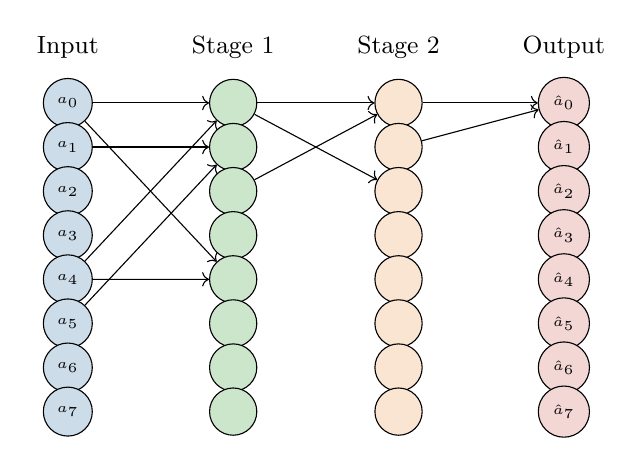
\begin{tikzpicture}[scale=0.7]
    % Input
    \foreach \i in {0,...,7} {
        \node[circle, draw, fill=primaryblue!20, minimum size=0.6cm] (a\i) at (0, -\i*0.8) {\tiny $a_\i$};
    }
    
    % Stage 1
    \foreach \i in {0,...,7} {
        \node[circle, draw, fill=secondarygreen!20, minimum size=0.6cm] (b\i) at (3, -\i*0.8) {};
    }
    
    % Stage 2
    \foreach \i in {0,...,7} {
        \node[circle, draw, fill=accentorange!20, minimum size=0.6cm] (c\i) at (6, -\i*0.8) {};
    }
    
    % Output
    \foreach \i in {0,...,7} {
        \node[circle, draw, fill=hardwarered!20, minimum size=0.6cm] (d\i) at (9, -\i*0.8) {\tiny $\hat{a}_\i$};
    }
    
    % Butterfly connections (simplified)
    \draw[->] (a0) -- (b0);
    \draw[->] (a4) -- (b0);
    \draw[->] (a0) -- (b4);
    \draw[->] (a4) -- (b4);
    
    \draw[->] (a1) -- (b1);
    \draw[->] (a5) -- (b1);
    
    \draw[->] (b0) -- (c0);
    \draw[->] (b2) -- (c0);
    \draw[->] (b0) -- (c2);
    
    \draw[->] (c0) -- (d0);
    \draw[->] (c1) -- (d0);
    
    % Labels
    \node at (0, 1) {\small Input};
    \node at (3, 1) {\small Stage 1};
    \node at (6, 1) {\small Stage 2};
    \node at (9, 1) {\small Output};
\end{tikzpicture}
\end{center}

\begin{infobox}[NTT Parallelism]
Each NTT stage has $n/2$ independent butterfly operations. GPUs process these in parallel; FPGAs pipeline them for streaming throughput.
\end{infobox}

% ============================================
% CHAPTER 9: Conclusion
% ============================================

\chapter{Conclusion and Future Directions}

\section{Key Takeaways}

\begin{enumerate}[leftmargin=*]
    \item \textbf{Quantum Threat}: Shor's algorithm breaks RSA/ECC; Grover weakens symmetric crypto. Migration to PQC is urgent.
    
    \item \textbf{NIST Standards}: ML-KEM, ML-DSA, SLH-DSA, and FN-DSA provide standardized post-quantum security.
    
    \item \textbf{Performance Challenge}: PQC algorithms have larger keys and higher computational costs than classical cryptography.
    
    \item \textbf{GPU Acceleration}: Massive parallelism enables batch processing; ideal for servers and data centers.
    
    \item \textbf{FPGA Acceleration}: Custom pipelines offer low latency and energy efficiency; ideal for embedded and networking.
    
    \item \textbf{Compression + PQC}: Hardware-accelerated compression reduces the bandwidth impact of larger PQC keys.
\end{enumerate}

\section{Future Trends}

\begin{center}
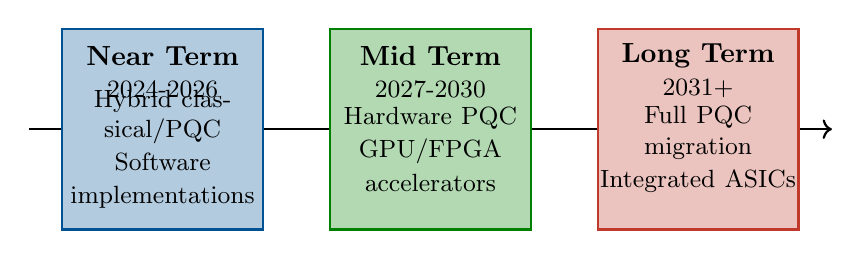
\begin{tikzpicture}[scale=0.85]
    % Timeline
    \draw[thick, ->] (0,0) -- (12,0);
    
    % Near term (2024-2026)
    \fill[primaryblue!30] (0.5,-1.5) rectangle (3.5,1.5);
    \draw[primaryblue, thick] (0.5,-1.5) rectangle (3.5,1.5);
    \node at (2,1.1) {\textbf{Near Term}};
    \node at (2,0.6) {\small 2024-2026};
    \node[text width=2.5cm, align=center] at (2,-0.3) {\small Hybrid classical/PQC\\Software implementations};
    
    % Mid term (2027-2030)
    \fill[secondarygreen!30] (4.5,-1.5) rectangle (7.5,1.5);
    \draw[secondarygreen, thick] (4.5,-1.5) rectangle (7.5,1.5);
    \node at (6,1.1) {\textbf{Mid Term}};
    \node at (6,0.6) {\small 2027-2030};
    \node[text width=2.5cm, align=center] at (6,-0.3) {\small Hardware PQC\\GPU/FPGA accelerators};
    
    % Long term (2031+)
    \fill[hardwarered!30] (8.5,-1.5) rectangle (11.5,1.5);
    \draw[hardwarered, thick] (8.5,-1.5) rectangle (11.5,1.5);
    \node at (10,1.1) {\textbf{Long Term}};
    \node at (10,0.6) {\small 2031+};
    \node[text width=2.5cm, align=center] at (10,-0.3) {\small Full PQC migration\\Integrated ASICs};
\end{tikzpicture}
\end{center}

\subsection{Emerging Technologies}

\begin{itemize}[leftmargin=*]
    \item \textbf{PQC ASICs}: Custom chips for specific PQC algorithms
    \item \textbf{In-memory Computing}: Process data where it resides
    \item \textbf{Photonic Accelerators}: Optical computing for NTT operations
    \item \textbf{Quantum-Safe HSMs}: Hardware security modules with PQC support
\end{itemize}

\section{Recommendations}

\begin{warningbox}
Organizations should begin planning PQC migration \textbf{now}. The ``Harvest Now, Decrypt Later'' threat means sensitive data encrypted today may be compromised in the future.
\end{warningbox}

\subsection{Implementation Roadmap}

\begin{enumerate}[leftmargin=*]
    \item \textbf{Inventory}: Catalog all cryptographic assets and dependencies
    \item \textbf{Prioritize}: Focus on long-lived secrets and critical systems
    \item \textbf{Test}: Evaluate PQC algorithms for performance and compatibility
    \item \textbf{Hybrid}: Deploy hybrid classical/PQC solutions initially
    \item \textbf{Monitor}: Track NIST guidance and quantum computing advances
    \item \textbf{Accelerate}: Implement hardware acceleration where needed
\end{enumerate}

\section{Summary Table}

\begin{table}[h]
\centering
\caption{Technology Selection Guide}
\begin{tabular}{@{}lll@{}}
\toprule
\textbf{Use Case} & \textbf{Recommended} & \textbf{Rationale} \\
\midrule
Server/Cloud & GPU (CUDA) & High throughput, batch processing \\
Networking & FPGA & Low latency, inline processing \\
Embedded/IoT & FPGA & Power efficiency, small footprint \\
General Purpose & CPU + Software & Flexibility, ease of deployment \\
Hybrid Systems & GPU + FPGA & Combine throughput and latency \\
\bottomrule
\end{tabular}
\end{table}

\begin{keypoint}
The transition to post-quantum cryptography is not optional---it is a necessary evolution. Hardware acceleration will be essential to maintain performance in a post-quantum world.
\end{keypoint}

\vspace{1cm}

\begin{center}
\textit{``The quantum revolution in computing necessitates a quantum revolution in cryptography.''}
\end{center}

\end{document}
